\documentclass{article}
\usepackage{import}
\subimport{../}{preamble}
\begin{document}

\section{Plasmons}
\label{sec:plasmons}

Plasmons are a direct solution of Maxwell's equations at the boundary between a dielectric and a metal. Despite existing on length scales from \SI{100}{nm} down to around \SI{1}{nm}, the high free electron density of metals mean energy levels still retain their characteristic continuous conduction bands and quantisation effects can be ignored.%
\footnote{A higher density of states means that energy levels are more closely spaced, hence metals with a large free electron density appear to have an energy continuum as opposed to discrete energy bands or levels at room temperature.}
Hence, classical theory is able to accurately describe physical phenomena until the characteristic length scale drops below $\sim$\SI{0.5}{nm} and a phenomenological approach using Maxwell's equations forms the basis of the mathematical description of plasmons.

\subsection{Electromagnetic Waves}
\label{sec:em_waves}

Maxwell's equations universally describe the classical, dynamical behaviour of \gls{em} waves, representing the foundations of electromagnetism. In their macroscopic, differential form, describing EM fields in matter, they are given by,
\begin{subequations}
\begin{align}
	\nabla \cdot \vec{D} &= \rhoext, \label{eq:maxwell1}\\
	\nabla \cdot \vec{B} &= 0, \label{eq:maxwell2}\\
	\nabla \times \vec{E} &= -\frac{\partial \vec{B}}{\partial t}, \label{eq:maxwell3}\\
	\nabla \times \vec{H} &= \Jext + \frac{\partial \vec{D}}{\partial t}, \label{eq:maxwell4}
\end{align}
\end{subequations}
where \gls{E} is the electric field, \gls{B} is the magnetic flux density, \gls{D} is the electric displacement field, \gls{H} is the magnetic field, \gls{rho_ext} is the free (volume) charge density, \gls{J_ext} is the free current density and \gls{t} is time. The charge and current densities refer to only the external contributions from free charges, related to the internal contributions from bound charges via $\gls{rho_tot}=\rhoext+\gls{rho_int}$ and $\gls{J_tot}=\Jext+\gls{J_int}$. \vec{D} and \vec{H} are introduced to include material dependencies and describe macroscopic fields, and are defined by,
\begin{subequations}
\begin{align}
	\vec{D} &= \epsfs\vec{E} + \vec{P}, \label{eq:displacement_field}\\
	\vec{H} &= \frac{1}{\mu_0}\vec{B} + \vec{M}, \label{eq:magnetic_field}
\end{align}
\end{subequations}
where \gls{P} is the polarisation (dipole moment per unit volume), \gls{M} is the magnetisation, and \gls{eps0} and \gls{mu0} are the permittivity and permeability of free space, respectively. For linear media, microscopic and macroscopic fields are related through the constitutive relations,
\begin{align}
	\vec{D} &= \eps\epsfs\vec{E}, \label{eq:fourier_displacement_field}\\
	\vec{H} &= \frac{1}{\mu\mu_0}\vec{B},
\end{align}
from which \gls{eps} and \gls{mu} are defined as the relative permittivity and permeability used to describe the electromagnetic properties of the medium.

The displacement field arises due to polarisation of a material in response to an applied field and is related to the internal charge density by $\nabla\cdot\vec{P}=\rhoint$. Conservation of charge means that $\nabla\cdot\vec{J}=\partial\rho/\partial t$, which requires that $\vec{J}=\partial\vec{P}/\partial t$ (a result also achievable by differentiating \eqref{eq:displacement_field}). The final equation of importance is the relationship between the electric field and the current density, given by,
\begin{equation}
	\vec{J} = \sigma\vec{E},
	\label{eq:current_density}
\end{equation}
where \gls{conductivity} is the conductivity. These few relations are sufficient to understand the behaviour of electromagnetic waves in media.

% Wave equation
Propagation of EM waves within a medium is governed by a wave equation relating both the spatial and temporal changes of a wave. Combining \eqref{eq:maxwell3} and \eqref{eq:maxwell4} leads to the general wave equation for EM waves in the time domain,
%\footnote{Derived using $\nabla \times \nabla \times \vec{E} = \nabla(\nabla\cdot\vec{E}) - \nabla^2\vec{E}$}%
\begin{align}
	\nabla(\nabla\cdot\vec{E}) - \nabla^2\vec{E} &= -\eps\epsfs\mu\mu_0\frac{\partial^2\vec{E}}{\partial t^2} - \mu\mu_0\gls{J},% \\
	%\nabla(\nabla\cdot\gls{D}) - \nabla^2\gls{D} &= \frac{\partial^2\gls{D}}{\partial t^2} - \Jext,
	\label{eq:wave_equation}
\end{align}
describing the propagation of an EM wave in a given medium.
In the absence of both charge and current \eqref{eq:wave_equation} reduces to,
\begin{equation}
	\nabla^2\vec{E} = \eps\epsfs\mu\mu_0\frac{\partial^2\vec{E}}{\partial t^2},
\end{equation}
describing a wave propagating in both space and time with a velocity $\gls{v}=1/\sqrt{\epsfs\eps\mu_0\mu}$. In free space ($\eps=\mu=1$) this is the speed of light $\gls{c}=1/\sqrt{\epsfs\mu_0}$, with light slowed when in media to $v=c/\refind$ by a factor $\gls{refractive_index}=\sqrt{\eps\mu}$ known as the refractive index.

% Relate to plasmons
In general \eps\ is a complex quantity, $\eps=\eps_1+i\eps_2$, and depends on the frequency of the EM wave, \gls{omega}. Plasmons are a phenomenon resulting from this frequency dependence in metallic materials. The relative permittivity is therefore denoted \dielectric\ and is referred to as the material's dielectric function from this point onwards. The concept of a plasmon can be identified through this function alone. Equations are therefore simplified by setting $\mu=1$ and removing any magnetic contributions.
% refractive index
Since \dielectric\ is a complex parameter with components $\eps_1+i\eps_2$, the complex refractive can be expressed as $\refind=\sqrt{\dielectric}=n+i\kappa$, where $n$ is the real part causing refraction and $\kappa$ is the loss coefficient determining absorption in the medium. The complex refractive index and the dielectric function are then related via $\eps_1=n^2-\kappa^2$ and $\eps_2 = 2n\kappa$.

The dispersive properties of a material are found by solving \eqref{eq:wave_equation} with $\eps=\dielectric$, describing the behaviour of a wave propagating through a non-magnetic, dielectric medium. For a propagating EM wave with frequency $\omega$ and wave vector \gls{wavevector} in space \gls{rv} of the form,
\begin{equation}
	\vec{E} = \gls{E0} \e^{i(\wv \cdot \vec{r} - \omega t)},
	\label{eq:wave}
\end{equation}
\eqref{eq:wave_equation} can be expressed in the frequency (Fourier) domain as,
%\footnote{Derived using the identities $\nabla \times \nabla \times \vec{E} = \nabla(\nabla\cdot\vec{E}) - \nabla^2\vec{E}$, $\nabla^2\vec{E}=-\wvm^2\vec{E}$ and $\partial^2\vec{E}/\partial t^2 = -\omega^2\vec{E}$ where $\nabla\cdot\vec{E}=0$}
\begin{equation}
	%\nabla(\nabla\cdot\vec{E}) - \nabla^2\vec{E} = -\eps(\wv, \omega) \frac{\omega^2}{c^2}\vec{E},
	\wv(\wv\cdot\vec{E}) - \wvm^2\vec{E} = -\eps(\wv, \omega) \frac{\omega^2}{c^2}\vec{E},
	\label{eq:fourier_wave_equation}
\end{equation}
where $\gls{wavevector_mag}=|\wv|$ is the magnitude of the wavevector. The variable $\gls{wavevector0} = \omega/c$ is sometimes used in \eqref{eq:fourier_wave_equation} when all quantities considered are wave vectors. From this equation the propagation behaviour of EM waves in media can be described.

Solutions to \eqref{eq:fourier_wave_equation} depend on the orientation of the wavevector with the field. Transverse wave solutions ($\wv\cdot\vec{E}=0$) yield the dispersion relation for light,
\begin{equation}
	\wvm = \sqrt{\eps(\wv, \omega)}\frac{\omega}{c}=\refind\wvz.
	\label{eq:light_dispersion}
\end{equation}
Inserting this into \eqref{eq:wave} gives a general solution for light propagating through a dielectric medium,
\begin{equation}
	\vec{E} = \vec{E}_0 \e^{\left({-\kappa\wvz r}\right)} \e^{\left[{i\left(n \wvz r - \omega t\right)}\right]}.
	\label{eq:gen_wave_solution}
\end{equation}
The real component of the refractive index $n$ slows the wave whereas the imaginary component corresponds to an exponential decay with characteristic length $1/\kappa$, representing loss within a medium.

Longitudinal wave solutions ($\wv\cdot\vec{E} = \wvm|\vec{E}|$) result in $\sqrt{\eps(\wv,\omega)}\omega/c = 0$, hence solutions only exists for $\eps(\wv, \omega)=0$. Both these conditions are important when describing plasmons in the bulk of a metal (only longitudinal plasmons are supported) and on the surface (both transverse and longitudinal plasmons supported).
%Furthermore, when considering the behaviour of \gls{em} waves at an interface between two different media the orientation of the fields with respect to the interface becomes important. Separate solutions exist depending on if a wave is considered \gls{tm} or \gls{te} (either only \vec{E} or \gls{H} has a component in the direction of propagation, respectively).%
%\footnote{\gls{te} and \gls{tm} are also known as $s$- and $p$-polarisations, respectively.}

Lastly, combining \eqref{eq:fourier_displacement_field} with the differential of \eqref{eq:displacement_field}, \eqref{eq:current_density} and \eqref{eq:wave}
%\footnote{$\partial/\partial t \rightarrow -i\omega$ and $\vec{J}=\dot{\vec{D}}-\epsfs\dot{\vec{E}}=\epsfs\dot{\vec{E}}(\eps-1)=\sigma\vec{E}$}
yields a relation between a material's conductivity and it's dielectric function,
\begin{equation}
	\eps(\wv, \omega) = 1 + \frac{i\sigma(\wv, \omega)}{\epsfs\omega}.
	\label{eq:dielectric_conductivity}
\end{equation}
Both quantities are able to describe the same physics from a different perspective.
%\footnote{Choice of which variable to use is a matter of convenience and tradition. Either can be used to equally describe the electromagnetic response of a material. The conductivity is typically used to describe lower frequency phenomena while the dielectric function is used at higher frequencies.}
Since \real{\eps} is related to both \imag{\sigma} and \real{\refind}, \real{\sigma} must therefore be related to $\kappa=\imag{\refind}$ and the attenuation of waves inside media. A large conductivity in a material corresponds to large transmission losses with decay attributed to the energy needed to move electrons at the surface of the material. Furthermore, the relation between \dielectric\ and $\sigma$ becomes important when considering points of conductance in a plasmonic system and that plasmons exist as an oscillating current density induced by a time-varying polarisation.

% Lead into the optical properties of metals
Using the framework outlined so far the optical properties of metals can be deduced along with the existence of plasmons. The discussion begins with the Drude model for the optical response of metals \cite{drude1900}, which is used to first predict the behaviour of plasmons. From there the distinction can be made between plasmons within the volume of a metal and those confined to the surface, which are of most interest in plasmonics.

\subsection{Bulk Plasmons and the Optical Properties of Metals}

% work on this paragraph
The optical properties of a metal are dominated by the response of highly mobile, nearly-free electrons delocalised from the positive nuclei background. When light is incident on a metal, nearly free electrons at the surface are displaced in the opposite direction to the field. The field of the induced charge distribution therefore screens the electric field inside the metal. Field penetration into the metal is strongly attenuated, with fields decaying exponentially over a characteristic ($1/2\e$) length known as the skin depth, $\gls{skin_depth} = c/2\omega\kappa$.%
\footnote{The skin depth is defined using $1/2\e$ rather than $1/\e$ to consider power instead of field.}
The small values of \skindepth\ exhibited by metals means that they fall within the \textit{perfect conductor} approximation (zero internal field) with transmission only possible through thin metallic films. An EM wave impinging on a metal is hence internally screened and reflected, giving metals their shiny appearance. A metal begins to show a more ``dielectric-like" behaviour when the frequency of incoming light is high enough that electron inertia prohibits an instantaneous response, thus allowing field penetration. Such effects are seen in the visible region of the \gls{em} spectrum in the case of noble metals. Fields increasingly penetrate metals up until \gls{uv} photon energies, at which point most metals become transparent. This is known as the \textit{ultraviolet transparency}.

% Defining the dielectric function of a metal and discerning the plasma frequency (volume plasmons)
Since the dominating cause of these effects stems almost exclusively from nearly free electrons, as opposed to bound electrons,%
\footnote{Optical properties derived from bound electrons are described by a Lorentz oscillator model.}
the optical properties of metals can be classically described by the Drude model \cite{drude1900}. This model describes the motion of a free electron gas in response to an applied field. The equation of motion for a single free electron in a time-varying applied field is given by,
\begin{equation}
	m\ddot{\vec{r}}(t) + m\gamma \dot{\vec{r}}(t) = -e\vec{E}(t),
\end{equation}
where \gls{m} is its effective optical mass, $e$ its charge, and $\gls{gamma} = 1/\tau$ its electron collision frequency, the inverse of the relaxation time, \gls{tau}. Using an effective optical mass as opposed to the actual electron mass incorporates band structure effects into the model. The electron collision frequency amounts to an effective coefficient of damping as in a mechanical oscillator. For a harmonic driving field, the induced oscillatory response of the free electrons induces a polarisation ($\vec{P} = -ne\vec{r}$, where \gls{n} is the number density of electrons),
\begin{equation}
	\vec{P}(t) = -\frac{ne^2}{m(\omega^2 + i\gamma\omega)}\vec{E}(t).
	\label{eq:P_solution}
\end{equation}
The resulting displacement field, obtained by substituting \vec{P} into \eqref{eq:displacement_field} and using \eqref{eq:fourier_displacement_field}, defines the dielectric function of a metal,
\begin{equation}
	\eps(\omega) = 1 - \frac{\omegap[2]}{\omega^2 + i\gamma\omega},
	\label{eq:basic_dielectric_function}
\end{equation}
where \gls{omega_p} is the plasma frequency of the metal, given by,
\begin{equation}
	\omegap[2] = \frac{ne^2}{\varepsilon_0 m}.
	\label{eq:plasma_frequency}
\end{equation}
The optical properties of a metal can be discerned from the real and imaginary components of \dielectric. The plasma frequency defines the point at which a metal transitions into a dielectric. For $\omega<\omegap$, $\real{\eps(\omega<\omegap)} < 0$ and a free electron gas remains metallic in character, with electrons moving to oppose an incident field. Once $\omega > \omegap$ the free electron gas, limited by inertia, cannot respond fast enough to the field and the metal becomes dielectric in character. In real metals, interband transitions increase \imag{\dielectric} and \eqref{eq:basic_dielectric_function} has to be modified to account for interband absorption caused by bound electrons through the inclusion of a constant $\eps_\infty$. The dielectric function then has the form,
\begin{equation}
	\dielectric = \eps_\infty - \frac{\omegap[2]}{\omega^2 + i\gamma\omega}.
	\label{eq:dielectric_function}
\end{equation}

\begin{figure}[bt]
\centering
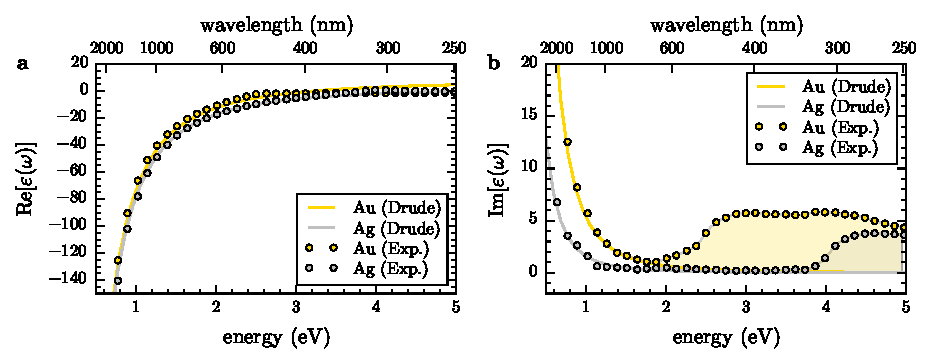
\includegraphics{figures/dielectric_function}
\caption[Plot of the dielectric function, given by the Drude model, for Au and Ag compared with empirical data]{\textbf{Plot of the dielectric function, given by the Drude model, for Au and Ag compared with empirical data.} \dielectric\ is calculated using \eqref{eq:dielectric_function}. The plasma frequency is calculated using \eqref{eq:plasma_frequency}. The parameters of the curves are $n=\SI{5.90e28}{\per\metre\cubed}$, $m=\SI{9.11e-31}{kg}$, $\gamma=1/\tau=1/\SI{1e-14}{s}$ and $\eps_\infty = 8$ for Au and $n=\SI{5.86e28}{\per\metre\cubed}$, $m=\SI{9.11e-31}{kg}$, $\gamma=1/\tau=1/\SI{3e-15}{s}$ and $\eps_\infty = 3$ for Ag. Empirical data (Johnson and Christy, 1972 \cite{johnson1972optical}) is shown for comparison to illustrate the importance of interband transitions. Differences between the Drude model (solid lines) and experimental results (circles) are caused by interband transitions not included in the basic Drude formalism.}
\label{fig:dielectric_function}
\end{figure}

A plot of \eqref{eq:dielectric_function} is shown in \figurename~\ref{fig:dielectric_function} , along with empirical data, illustrating both why noble metals exhibit high quality, visible spectrum (400--\SI{700}{nm}, 1.5--\SI{3}{eV}) plasmonics, as well as the failings of the Drude model. Noble metals have $\real{\dielectric}<0$ and small \imag{\dielectric} in the visible region, hence behave very similarly to an ideal free electron gas. The Drude model fails at higher energies as interband transitions are not included in the basic model. These transitions increase the absorption ($\propto\imag{\dielectric}$) and are significant for $\lambda < \SI{500}{nm}$ in Au and $\lambda<\SI{300}{nm}$ in Ag. A measure of the quality of a metal can be determined from its quality factor $\gls{Q} = \left|\real{\eps}/\imag{\eps}\right|$. The high $Q$ of noble metals in the visible regions means they can easily respond to an incident field and screen it, behaving metallically.

%\begin{figure}[bt]
%\centering
%\fontsize{10pt}{1em}\selectfont
%\subimport{./figures/}{bulk_charge_displacement.pdf_tex}
%\caption[Charge displacement of a free electron gas under an applied field]{\textbf{Charge displacement of a free electron gas under an applied field.} The optical electric field displaces the electrons leaving behind the positive cores. The slab becomes polarised with opposing surface charge densities $\sigma$. The charge oscillations resonate when the field frequency is \omegap.}
%\label{fig:bulk_charge_displacement}
%\end{figure}

The plasma frequency \omegap\ in \dielectric\ not only describes a metal-to-dielectric transition but also dictates the frequency of the collective longitudinal mode of oscillation. By substituting \eqref{eq:basic_dielectric_function} in the zero damping limit into the dispersion relations for transverse and longitudinal waves it is clear that transverse waves are only supported if $\omega>\omegap$ with a dispersion $\omega^2=\omegap[2]+\wvm^2c^2$. However, a collective longitudinal oscillation is allowed at $\omega=\omegap$ since $\dielectric=0$ in the absence of damping. In this case the free electron gas is displaced from the ionic core background a distance \gls{u} due to the applied field to form surface charge densities $\gls{sigma} = \pm neu$. The resulting depolarisation field
%\footnote{Gauss' law $\int \vec{E}\cdot d\vec{A} = Q/\epsfs=\sigma A/\epsfs$, hence $E=\sigma/\epsfs$. Alternatively $D=0=\epsfs\vec{E}+\vec{P}$ therefore $\vec{E}=-\vec{P}/\epsfs=-ne\vec{u}/\epsfs$.}
is $E = neu/\epsfs$ and the motion of the free electrons is defined by,
\begin{equation}
	nm\ddot{u} = -neE = -\frac{n^2e^2u}{\epsfs}.
\end{equation}
Simplifying this relation leads to,
\begin{equation}
	\ddot{u}+\omegap[2] u=0,
\end{equation}
hence \omegap\ is considered the natural frequency of the system and the electrons resonate when driven at $\omega=\omegap$. This is known as the bulk or \emph{volume plasmon}. Since this is a longitudinal oscillation, however, light cannot couple with it. For this reason, volume plasmons cannot be excited and measured by means of optical techniques but require other experimental methods, e.g.\ \gls{eels} \cite{egerton2011electron}. Optical plasmonic phenomena must therefore be a result of a different kind of plasmon.

\subsection{Surface Plasmons}
% EELS of LSPs nelayah2007, koh2009, duan2012

\Glspl{sp}, unlike bulk plasmons, are collective oscillations of conduction electrons tightly confined to the surface of the metal and therefore not necessarily restricted by the diffraction limit. The maximum magnitude of the wavevector is set by $\wvz=2\pi/\lambda$ with individual components restricted by $\wvm = \sqrt{\wvm_x^2 + \wvm_y^2 + \wvm_z^2}$. Consider \eqref{eq:light_dispersion} in the form,
\begin{equation}
	\wvm_x^2 = \refind^2 \wvz^2 - \wvm_y^2 - \wvm_z^2.
\end{equation}
If a wave propagates freely in all three dimensions then it remains diffraction limited and the propagation constant $\wvm_x < \refind\wvz$. However if one or more of its wavevector components become imaginary ($\wvm_{y,z}^2 < 0$) then it becomes possible that $\wvm_x > \refind\wvz$. This behaviour can occur at an interface, where surface waves take on evanescent character in the $z$-direction whilst propagating in the $xy$ plane.%
\footnote{Evanescent meaning imaginary $\wvm_z$ therefore exponentially decaying amplitude in the $z$-direction.}
By coupling light into surface waves the diffraction limit can be beaten. Waves of frequency $\omega$ can acquire wavelengths many times smaller than their excitation wavelength. The SP is one such case of this phenomenon and occurs at metal-dielectric interfaces. Unlike in a bulk metal, electrons displaced by an applied field at the surface of a metal feel a restoring force due to the positive nuclei background. Transverse fields impinging on the metal surface at an angle are then able to manipulate the electron motion. SPs can therefore be excited by light as well as by the longitudinal waves needed to excite bulk plasmons, forming polariton quasiparticles under strong coupling with photons.%
\footnote{Polaritons are the name given to quanta or quasiparticles of light-matter interactions. Strong coupling describes the point at which a quasiparticle is no longer distinguishable between its two constituent components.}
This optical excitation is known as the \gls{spp} and, as a result of it being optically accessible, is one of the most commonly studied plasmonic phenomenons.

\subsubsection{Surface Plasmon Polaritons}

\begin{figure}[bt]
\fontsize{10pt}{1em}\selectfont
\def\svgwidth{0.6\textwidth}
\subimport{./figures/}{spp_diagram.pdf_tex}
\caption[Diagram of a surface plasmon polariton (SPP)]{\textbf{Diagram of a surface plasmon polariton (SPP).} TM surface electron density waves (surface plasmons) couple with an evanescent wave originating from an EM wave to form a SPP. The SPP remains confined to the interface but can propagate across the surface.}
\label{fig:spp_diagram}
\end{figure}

An SPP is a propagating \gls{tm} wave confined to the surface of a metal - the bound state between a photon and a SP. The TM nature of the wave indicates that \vec{E} has a component traversing across the interface as shown in the diagram of an SPP in \figurename~\ref{fig:spp_diagram}. No such solution exists for \gls{te} surfaces waves (i.e.\ a component of \vec{H} passing through the interface).%
\footnote{TE and TM are also known as $s$- and $p$-polarisations, respectively.}
While confined in two dimensions to the planar boundary between a metal and a dielectric, the SPP can either propagate or become stationary as a result of interference. The latter stationary form of the SPP is similar to the localised surface plasmons, described later.

The SPP itself is described through its dispersion. A TM wave propagating in the $x$-direction along a metal/dielectric interface has a spatial field profile in a space \vec{r} given by $\vec{E}(\vec{r}) = \vec{E}(z)\e^{i\beta x}$ where $\beta=\wvm_x$ is the propagation constant. The magnetic field in this configuration is then $\vec{H}(\vec{r}) = \vec{H}(y)e^{i\beta x}$. Solving the wave equation across the metal-dielectric interface leads to the dispersion relation of a SPP, given by,
\begin{equation}
	\beta = \frac{\omega}{c}\sqrt{\frac{\epsdi\dielectric}{\epsdi + \dielectric}}.
	\label{eq:spp_dispersion}
\end{equation}
\begin{figure}[bt]
\centering
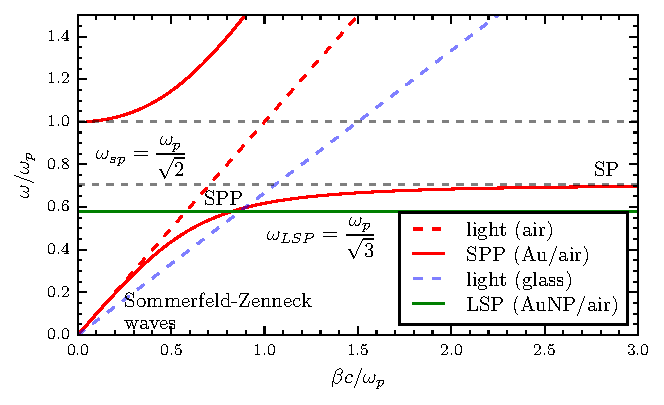
\includegraphics{figures/spp_dispersion}
\caption[Plasmon dispersion relations for the SPP and LSP]{\textbf{Plasmon dispersion relations for the SPP and LSP.} The dashed lines indicate the dispersion of light in both glass and air (vacuum) along with the surface plasmon frequency. SPPs can be described as photon-like or plasmon-like depending on their point of excitation. SPPs excited with large \wvm\ and $\omega\approx\omega_{SPP}$ are considered plasmon-like while SPPs with low \wvm\ are considered more photon-like. These have been known as Sommerfeld-Zenneck surface waves \cite{kittel1976introduction}.}
\label{fig:spp_dispersion}
\end{figure}
This dispersion is shown in \figurename~\ref{fig:spp_dispersion} along with the dispersion of light for both air and glass mediums.
% Excitation of SPPs
From the dispersion curve it is clear that SPPs cannot couple with light within the same medium as their dispersion curves do not cross. However, light from within a higher refractive index medium such as glass can generate evanescent waves and excite SPPs on a nearby metal/air interface. This method of coupling photons with surface plasmons, depending on the specific prism arrangement, is known as the Kretschmann (prism-metal-dielectric) or Otto (prism-dielectric-metal) configuration \cite{otto1968, kretschmann1971}. Since a diffraction grating may also impart momentum onto a photon ($\wvm_x \rightarrow \wvm_x + n\pi$) a metallic grating can launch SPPs along a planar metal-dielectric interface. This phenomenon was first observed in 1902 by Wood, dubbed as Wood's anomaly \cite{wood1902}, and only explained via surface waves many years later \cite{fano1941}.

% Plasmon property: nm-scale wavelength with visible frequency
Closer inspection of the curve highlights one of the major features of a plasmon. While SPPs retain the frequency of the excitation field, their wavelength is considerably smaller than the diffraction-limited wavelength of light.
% photon-like vs plasmon-like
Depending on where on the curve the SPP lies it can be considered to be either more photon-like or more plasmon-like. For small $\beta\approx\wvz$ the SPP is similar to light grazing the interface (Sommerfeld-Zenneck waves)%
\footnote{Sommerfeld-Zenneck waves are surface waves that appear throughout mechanics and electromagnetism that are confined to the interface between two different mediums.}
whereas SPPs with large \wvm\ become more plasmon-like and their frequency saturates at the surface plasmon frequency,
\begin{equation}
	\omegasp = \frac{\omegap}{\sqrt{1+\epsdi}}.
\end{equation}
At this point the SPP can be considered electrostatic and becomes an SP. To some extent, SPs confined to a finite, continuous, non-planar surface, defining a \gls{mnp}, can be considered to be the basis for \glspl{lsp} or \glspl{lspp}.

\subsubsection{Localised Surface Plasmons}

% Localised Surface Plasmons
LSPs are collective oscillations of conduction electrons confined within a fixed sub-wavelength spatial extent. These can occur on any nanoscale curved surface but the effects are strongest, and most well-documented, on the surface of a MNP. Free electrons are displaced from the nuclei in response to an applied field and form a surface charge distribution, polarising the particle. Coulomb interaction between the poles of the surface charge distribution results in a restoring force on electrons within the particle. This gives rise to a natural frequency of oscillation, leading to resonance when driven harmonically at the correct frequency. The particular resonant frequencies present in a particle depend on the particle geometry (supporting various multipolar surface charge distributions), its material properties and the dielectric properties of the surrounding medium, which each modify the electron restoring forces. Each different multipolar charge distribution is considered to be a unique LSP mode, identifiable by its optical resonance \cite{murray2007}.

\begin{figure}[bt]
\centering
\fontsize{10pt}{1em}\selectfont
\def\svgwidth{0.35\textwidth}
\subimport{./figures/}{sphere_plasmon.pdf_tex}
~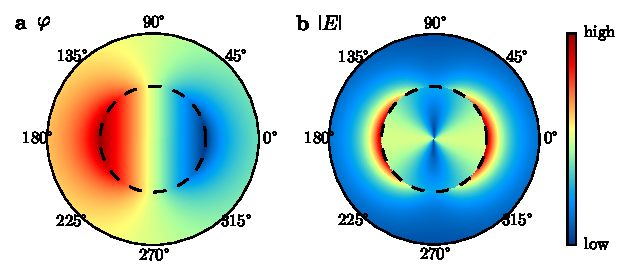
\includegraphics[width=0.59\textwidth]{figures/spherical_np_dipole_lsp}
\caption[A spherical metallic particle in an applied electric field]{\textbf{A spherical metallic particle in an applied electric field.} The sphere is assumed to in the quasistatic regime ($a\ll\lambda$). The aura around the particle indicates the phase of the free electron oscillations in the plasmon. Calculations of (a) the potential and (b) the magnitude of the electric field for a spherical nanoparticle on resonance ($\dielectric=-2\epsdi$).}
\label{fig:sphere_plasmon}
\end{figure}

The simplest form of a LSP is the dipole resonance of a spherical MNP. Assuming the sphere radius $\gls{a}\ll\lambda$ (the wavelength of light), the particle is considered to be in the quasistatic regime, where electrons move instantaneously in response to the incident field and their phase is ignored. Electrostatics, rather than electrodynamics, is applicable to solve this problem with an electrostatic potential, \gls{potential},  described by the Laplace equation, $\nabla^2\pot=0$. A general solution in a spherical geometry is of the form \cite{maier2007plasmonics},
\begin{equation}
	\pot_{l,m_l}(r,\theta,\phi) = \sum_{l=0}^{l=\infty} \sum_{m_l=-l}^l [ A_lr^l + B_lr^{-(l+1)} ] P_l^m (\cos\theta) \e^{i m_l\phi},
\end{equation}
where \gls{l} is the degree of spherical harmonic and \gls{m_l} its order, $A_l$ and $B_l$ are constants and $P_l^m(\cos\theta)$ are associated Legendre polynomials. For a sphere of radius $a$ and dielectric function \dielectric\ in a dielectric medium described by \epsdi\ the solution is fixed by boundary conditions, reducing to \cite{jackson1999classical},
\begin{equation}
	\pot =
	\begin{dcases}
	-\frac{3\epsdi}{\dielectric + 2\epsdi} \vec{E}_0\cdot\vec{r} & r \leq a\text{ (inside)}, \\
	\left(-1 + \frac{\dielectric - \epsdi}{\dielectric + 2\epsdi} \frac{a^3}{r^3}\right) \vec{E}_0\cdot\vec{r} & r > a\text{ (outside)}.
	\end{dcases}
\end{equation}
For a metal sphere the potential (plotted in \figurename~\ref{fig:sphere_plasmon}a) describes an induced dipolar surface charge distribution. The description is simplified by defining the dipole moment,
\begin{equation}
	\vec{p} = \epsfs\epsdi\alpha\vec{E}_0 = 4\pi\epsfs\epsdi a^3 \frac{\dielectric - \epsdi}{\dielectric + 2\epsdi} \vec{E}_0,
\end{equation}
where the polarisability, \gls{alpha}, incorporates the frequency dependent behaviour and is defined as,
\begin{equation}
	\alpha(\omega) = 4\pi a^2 \frac{\dielectric - \epsdi}{\dielectric + 2\epsdi}.
	\label{eq:polarisability}
\end{equation}
The outside potential is then expressed as,
\begin{equation}
	\pot_{out} = -\vec{E}_0\cdot\vec{r} + \frac{\vec{p}\cdot\vec{r}}{4\pi\epsfs\epsdi r^3}.
\end{equation}
This is simply the potential of an induced dipole superimposed onto the incident field. The electric field inside and outside of the sphere is calculated using $\vec{E}=-\nabla\pot$ and given by,
\begin{equation}
	\vec{E} =
	\begin{dcases}
	\frac{3\epsdi}{\dielectric+2\epsdi} \vec{E}_0 & r \leq a\text{ (inside)}, \\
	\vec{E}_0 + \frac{3\vec{n}(\vec{n}\cdot\vec{p}) - \vec{p}}{4\pi\epsfs\epsdi}\frac{1}{r^3} & r > a\text{ (outside)},
	\end{dcases}
	\label{eq:E_out}
\end{equation}
where $\vec{n}=\vec{r}/r$ is the radial unit vector, and shows a similar dipolar phenomenon as seen in \figurename~\ref{fig:sphere_plasmon}b.

Provided that the quasistatic approximation remains valid, the electrostatic result is simply multiplied with a harmonic time dependence to describe electrodynamic behaviour. Hence, an EM wave induces a coherent, oscillating dipole moment $\vec{p}\e^{i\omega t}=\epsfs\epsdi\alpha(\omega)\vec{E_0}\e^{i\omega t}$. The behaviour of electrons in the spherical MNP at optical frequencies, described using the dielectric function \dielectric, is then simply incorporated into $\alpha(\omega)$. For a good metal $\real{\dielectric}<0$ and the denominator in \eqref{eq:polarisability} undergoes resonance
%\footnote{$\alpha\rightarrow-\infty$ when $\dielectric+2\epsdi\rightarrow0$}
at the Fr\"{o}hlich condition when,
\begin{equation}
	\real{\dielectric} = -2\epsdi. \label{eq:frohlich}
\end{equation}
This corresponds to excitation of a collective oscillation of conduction electrons on the surface of the sphere - the dipolar LSP. Its magnitude in real metals is restricted by damping of the electron motion leading to a Lorentzian-shaped resonance band - the dipolar surface plasmon resonance. Its relationship with \epsdi\ means that the resonant frequency can be tuned by varying the external dielectric medium. As seen in \eqref{eq:E_out}, the field from the induced dipole moment of the plasmon is superimposed onto the incident field, leading to a resonant field enhancement both inside and outside the surface of the sphere. This is the single most useful property of a plasmon, and one that is heavily exploited in sensing and sensor developments.

In the Drude model, with \dielectric\ given by \eqref{eq:dielectric_function}, the Fr\"{o}hlich condition is satisfied when,
\begin{equation}
	\omegalsp = \frac{\omegap}{\sqrt{1+2\epsdi}},
\end{equation}
which evaluates to $\omega = \omegap/\sqrt{3}$ for a MNP in vacuum. As can be seen in \figurename~\ref{fig:spp_dispersion}, the flat dispersion of a LSP mode means it crosses the light line at a single point. Light of the correct frequency therefore readily couples with LSPs without the need for SPP momentum matching mechanisms.
% Spherical harmonics
In general, the optical spectrum of a MNP can contain a number of multipolar plasmon modes for which the resonant frequencies are given by \cite{prodan2004},
\begin{equation}
	\omega_l = \omegap\sqrt{\frac{l}{\epsdi(l+1)+1}},
\end{equation}
where $l$ denotes the charge distribution of a specific spherical harmonic mode ($l=1$ for dipole, $l=2$ for quadrupole, etc.). However, these modes only exist outside of the quasistatic regime in larger MNPs or more complex geometries.
% Link with noble metals
For nobles metals, such as Au and Ag, the fundamental $l=1$ mode occurs in the visible region of the EM spectrum ($\lambda=\SI{520}{nm}$ for Au and $\lambda=\SI{360}{nm}$ for Ag in vacuum or air \cite{maier2007plasmonics} and redshifted in the presence of other media \cite{sonnichsen2000}), leading to them often being the plasmonic metal of choice.
% geometry dependence
Additionally, the polarisability changes with MNP geometry due to differing restoring forces acting on the surface charge distribution. Changes from a spherical shaped MNP therefore lead to tuning of the LSP resonance across the visible spectrum. This geometrical dependence is well known \cite{krenn2000, mock2002, kuwata2003} and has been exploited in many applications over the past decade, e.g.\ \gls{ir} photothermal therapy \cite{huang2006, huang2008, huang2010gold}.

The larger the separation between opposing poles of surface charge, the weaker the restoring force. A larger particle, or similarly an elongated particle (a nanoellipsoid or nanorod), will therefore have lower energy resonances. Simple changes can be made to the theoretical (quasistatic) model to account for an ellipsoidal geometry, and thus somewhat understand the geometrical dependencies incorporated into the polarisability. Insertion of a geometrical correction to the polarisability leads to the definition \cite{maier2007plasmonics, noguez2007},
\begin{equation}
	\alpha_i(\omega) = 4\pi a_1a_2a_3\frac{\dielectric-\epsdi}{3\epsdi+3L_i(\dielectric-\epsdi)},
\end{equation}
where $i$ is the index of each anisotropic axis with a geometrical factor,
\begin{equation}
	L_i = \frac{a_1a_2a_3}{2}\int_0^\infty \frac{dq}{(a_i^2+q)\sqrt{(q+a_1^2)(q+a_2^2)(q+a_3^2)}}.
\end{equation}
The resonance condition along each axis then becomes,
\begin{equation}
	\real{\dielectric} = -\frac{1 - L_i}{L_i}\epsdi.
\end{equation}
By increasing the size of an axis, decreasing its associated geometrical factor, the resonance condition decreases from $\dielectric=-2\epsdi$, redshifting the resonant LSP frequency. The more elongated the particle becomes, the larger the redshift until the restoring force is weakened to the point that each LSP no longer exists.

\subsubsection{Optical Observation of Surface Plasmon Resonances}

Depending on the microscopic dipole moment of excited plasmons, their fields can be radiative and hence macroscopically observable. This depends on the geometry of the plasmons time-varying charge distribution. Antenna-like dipolar plasmons bear similarity with the Hertzian dipole, an infinitesimal oscillating current source which both absorbs and radiates EM waves. The relationship between the current, $\vec{I}(t)$, carried by the dipole of length $d$ and the radiative electric field around it is given by \cite{grant2013electromagnetism},
\begin{equation}
	\vec{E} = \frac{ik\vec{I}d\eta_o}{4\pi r} \e^{-ikr} \left[ \hat{r} \left( \frac{1}{ikr} + \frac{1}{(ikr)^2} \right) 2\cos\theta + \hat{\theta} \left( 1 + \frac{1}{ikr} + \frac{1}{(ikr)^2} \right) \sin\theta \right],
\end{equation}
The radial behaviour of the electric field around an object can be split into three distinct regimes - the \emph{near-field} or Fresnel regime and the \emph{far-field} or Fraunhofer regime. At short distances the $(\wvm r)^{-2}$ term dominates to form the near-field but quickly falls off with increasing distance. The remaining $(\wvm r)^{-1}$ term defines the far-field. The boundary between the near-field and the far-field is defined as the point at which $\wvm r=1$ where $r = \lambda/2\pi$ (hence why sub-wavelength optics deals with the near-field).

Plasmons similarly have the ability to both resonantly absorb and scatter incident fields. The absorbance and scattering cross sections determining interaction with a spherical MNP are given by \cite{bohren2008absorption},
\begin{subequations}
\begin{align}
	\gls{sigma_scat} &= \frac{\wvm^4}{6\pi} |\alpha|^2 = \frac{8\pi}{3}\wvm^4a^6 \left| \frac{\dielectric - \epsdi}{\dielectric + 2\epsdi} \right|^2, \\
	\gls{sigma_abs} &= \wvm\imag{\alpha} = 4\pi \wvm a^3 \imag{ \frac{\dielectric - \epsdi}{\dielectric + 2\epsdi} }.
\end{align}
\end{subequations}
Since $\sigma_{\mathrm{scat}} \propto V^2$ and $\sigma_{\mathrm{abs}} \propto V$, absorption dominates in smaller particles whilst larger particles scatter more strongly. The extinction cross section, commonly used in spectroscopy, can be calculated using $\gls{sigma_ext}=\sigma_{\mathrm{scat}}+\sigma_{\mathrm{abs}}$. The size of each cross-section, i.e.\ the spatial extent over which light interacts with the MNP, depends on $\alpha$ and is increased on resonance. Hence, MNPs optically appear strongly coloured and much larger than they actually are.%
\footnote{Consider that $\sigma_{\mathrm{scat}}$ for a AuNP is enhanced $100\times$ on resonance, meaning it's area cross-section is $\sqrt{100/\pi}= 6\times$ wider than it's radius, hence why a \SI{50}{nm} AuNP looks like a \SI{300}{nm} green sphere when imaged.}

For example, when on resonance with the dipolar LSP, both cross sections are enhanced by the polarisability resonance from the geometrical particle size to the \orderof{\SI{500}{nm}} scattering size. The increased size of the cross-section is comparable to the wavelength of light, meaning LSPs efficiently couple with photons in the far-field. The LSP mediates energy transfer between the near-field and the far-field and acts to match the electromagnetic modes of nanoscale absorbers/emitters, such as phonons (Raman) and radiative energy levels (quantum emitters, fluorescence), with those of a diffraction-limited photonic mode via an oscillating charge density \cite{berweger2012}. A plasmonic MNP is often therefore described as an \textit{optical antenna} in a similar manner to a device that converts between radio waves and an electrical current is named a radio antenna \cite{bharadwaj2009, novotny2011}. LSP modes which readily couple with the far-field are then sometimes referred to as \emph{antenna modes} and become important when designing resonant structures for specific sensing applications.

\begin{figure}[bt]
\centering
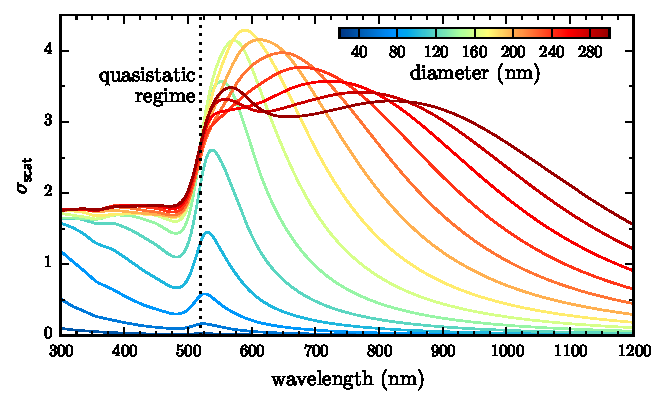
\includegraphics{figures/mie_scattering}
\caption[Mie scattering cross-sections for AuNPs of increasing diameter]{\textbf{Mie scattering cross-sections for AuNPs of increasing diameter.} The \SI{520}{nm} resonance position of the dipolar LSP mode of a AuNP in the quasistatic approximation is indicated by the dotted line. The resonance stays at \SI{520}{nm} until $d>\SI{80}{nm}$ then redshifts. The emergence of higher order modes following a similar behaviour is seen once $d>\SI{100}{nm}$.}
\label{fig:mie_scattering}
\end{figure}

Whilst the quasistatic approach is useful to first demonstrate the field enhancing capabilities of a MNP, the description breaks down once the size of the particle becomes closer to the excitation wavelength. Retardation effects result in phase differences between the incident field and the induced electron currents across the particle, which strongly influences the radiated fields. At this point Mie theory (electrodynamics) \cite{mie1908} is required to describe the spectral response of spherical MNPs, providing a more general description of their optical response. Using this approach the spectrum of a MNP can be decomposed into superimposed multipoles, arising from the existence of higher order LSP modes in larger MNPs with finite dipole moments. The spectral response of spherical AuNPs of varying sizes is shown in \autoref{fig:mie_scattering}, demonstrating the redshift and broadening of lower order modes with increasing particle size and the excitation of higher order modes.

% Lead into plasmon coupling
To summarise, by utilising the particle material, geometry and polarisation anisotropy, its LSPs can be tuned across the entire UV--NIR spectrum to tailor to individual applications. However, even when exciting on resonance, a single particle can only provide a relatively small field enhancement ($\left|E/E_0\right|\sim\orderof{5-10}$). An alternative approach to exploiting LSPs is therefore to couple the fields of many plasmons together. Through coupling, the confined fields in nanometric-size gaps between MNPs can be enhanced by many more orders of magnitudes.

\end{document}